% !Mode::"TeX:UTF-8"
% !Mode:: "TeX:UTF-8"
% \documentclass[xcolor=svgnames,table,10pt]{beamer}
\documentclass[10pt,aspectratio=43,mathserif]{beamer} 
\usepackage[orientation=landscape,size=custom,width=16,height=9,scale=0.3,debug]{beamerposter}
\usepackage{xeCJK}


\hypersetup{backref,pdfpagemode=FullScreen,colorlinks=true}

% 默认的数学公式较难看,使用serif可以使得公式的样式变为常用latex的公式样式 
\mode<presentation>{
% Setup appearance:
\usefonttheme[onlymath]{serif} 
\useoutertheme{infolines}
\usetheme{Darmstadt}
% \usetheme{Berlin} %主题
% \usetheme{Singapore}

\setbeamercovered{transparent}
\setbeamertemplate{caption}[numbered]
\setbeamertemplate{navigation symbols}{}
\setbeamertemplate{blocks}[rounded][shadow=true]
\setbeamertemplate{enumerate items}[circle]

% 修改样式
\setbeamercolor{box}{bg=black!20!orange,fg=white}
\setbeamercolor{block title}{use=sidebar,fg=sidebar.fg!10!white,bg=orange!70!black}
\setbeamercolor{block title example}{use=sidebar,fg=sidebar.fg!10!white,bg=black!60!green}
\setbeamercolor{block title alerted}{use=sidebar,fg=sidebar.fg!10!white,bg=black!50!red}

\setbeamertemplate{headline}
{%
  \begin{beamercolorbox}[shadow=true]{section in head/foot}
  \vskip2pt\insertnavigation{\paperwidth}\vskip2pt
  \end{beamercolorbox}%
}
}

\usepackage{url}
\usepackage{animate}
\usepackage[english]{babel}
\usepackage{times}
\usepackage[T1]{fontenc}
\usepackage{multirow,multicol,longtable}
\usepackage{graphics}
\usepackage{xcolor}
% \usepackage[no-math]{fontspec}%-------------------------------------------------- 提供字体选择命令
% \usepackage{xunicode}%----------------------------------------------------------- 提供Unicode字符宏
% \usepackage{xltxtra}%------------------------------------------------------------ 提供了针对XeTeX的改进并且加入了XeTeX的LOGO
% \usepackage[BoldFont,SlantFont,CJKchecksingle]{xeCJK}%--------------------------- 使用xeCJK宏包
%================================== 设置中文字体 ================================%
% \setCJKmainfont{Adobe Heiti Std}%------------------------------------------------设置正文为黑体
% \setCJKmonofont{Adobe Song Std}%-------------------------------------------------设置等距字体
% \setCJKsansfont{Adobe Kaiti Std}%------------------------------------------------设置无衬线字体
% \setCJKfamilyfont{zxzt}{FZShouJinShu-S10S}
% \setCJKfamilyfont{FZDH}{FZDaHei-B02S}
%================================== 设置中文字体 ================================%
% \hypersetup{backref,pdfpagemode=FullScreen,colorlinks=true}
% \hypersetup{pdfpagemode=FullScreen,colorlinks=true}

%================================== 设置英文字体 ================================%
% \setmainfont[Mapping=tex-text]{Times New Roman}%--------------------------------英文衬线字体
% \setsansfont[Mapping=tex-text]{Arial}%------------------------------------英文无衬线字体
% \setmonofont[Mapping=tex-text]{Courier New}%-------------------------------------英文等宽字体
% \newfontfamily\Arial{Arial}
%================================== 设置英文字体 ================================%

%================================== 设置数学字体 ================================%
%\setmathsfont(Digits,Latin,Greek)[Numbers={Lining,Proportional}]{Minion Pro}
%================================== 设置数学字体 ================================%

\punctstyle{kaiming}%------------------------------------------------------------ 开明式标点格式
\usepackage{graphicx}
\usepackage{tikz}
\usetikzlibrary{positioning,backgrounds}
\usetikzlibrary{fadings}
\usetikzlibrary{patterns}
\usetikzlibrary{calc}
\usetikzlibrary{shadings}
\pgfdeclarelayer{background}
\pgfdeclarelayer{foreground}
\pgfsetlayers{background,main,foreground}
\usepackage{xifthen}
\usepackage{colortbl,dcolumn}
\usepackage{enumerate}
\usepackage{pifont}
\usepackage{tabularx}
\usepackage{booktabs}
\usepackage[]{hyperref}
% \usepackage[colorlinks,linkcolor=blue]{hyperref}

% %代码设置
% \usepackage{listings}
% \usepackage{ctex}

% \lstset{
%     basicstyle          =   \sffamily,          % 基本代码风格
%     keywordstyle        =   \bfseries,          % 关键字风格
%     commentstyle        =   \rmfamily\itshape,  % 注释的风格,斜体
%     stringstyle         =   \ttfamily,  % 字符串风格
%     flexiblecolumns,                % 别问为什么,加上这个
%     numbers             =   left,   % 行号的位置在左边
%     showspaces          =   false,  % 是否显示空格,显示了有点乱,所以不现实了
%     numberstyle         =   \zihao{-5}\ttfamily,    % 行号的样式,小五号,tt等宽字体
%     showstringspaces    =   false,
%     captionpos          =   t,      % 这段代码的名字所呈现的位置,t指的是top上面
%     frame               =   lrtb,   % 显示边框
% }

% \lstdefinestyle{Python}{
%     language        =   Python, % 语言选Python
%     basicstyle      =   \zihao{-5}\ttfamily,
%     numberstyle     =   \zihao{-5}\ttfamily,
%     keywordstyle    =   \color{blue},
%     keywordstyle    =   [2] \color{teal},
%     stringstyle     =   \color{magenta},
%     commentstyle    =   \color{red}\ttfamily,
%     breaklines      =   true,   % 自动换行,建议不要写太长的行
%     columns         =   fixed,  % 如果不加这一句,字间距就不固定,很丑,必须加
%     basewidth       =   0.5em,
% }

%代码设置
\usepackage{fancybox}
\usepackage{color,xcolor}
\usepackage{times}
\usepackage{listings}

\definecolor{mygreen}{rgb}{0,0.6,0}
\definecolor{mygray}{rgb}{0.5,0.5,0.5}
\definecolor{mymauve}{rgb}{0.58,0,0.82}
\newcommand{\Console}{Console}
\lstset{ %
	backgroundcolor=\color{white},   % choose the background color
	basicstyle=\footnotesize\rmfamily,     % size of fonts used for the code
	columns=fullflexible,
	breaklines=true,                 % automatic line breaking only at whitespace
	captionpos=b,                    % sets the caption-position to bottom
	tabsize=4,
	commentstyle=\color{mygreen},    % comment style
	escapeinside={\%*}{*)},          % if you want to add LaTeX within your code
	keywordstyle=\color{blue},       % keyword style
	stringstyle=\color{mymauve}\ttfamily,     % string literal style
	numbers=left, 
%	frame=single,
	rulesepcolor=\color{red!20!green!20!blue!20},
	% identifierstyle=\color{red},
	language=c
}

% \usepackage[linesnumbered,ruled,lined]{algorithm2e}
% \usepackage{algorithm}  
% \usepackage{algorithmicx}  
% \usepackage{algpseudocode}
% \floatname{algorithm}{算法}
% \renewcommand{\algorithmicrequire}{\textbf{输入:}} 
% \renewcommand{\algorithmicensure}{\textbf{输出:}}  
% \algrenewcommand{\algorithmiccomment}[1]{ $//$ #1}

\usepackage{algorithm}  
\usepackage{algpseudocode}  
\usepackage{amsmath}  
\renewcommand{\algorithmicrequire}{\textbf{Input:}}  % Use Input in the format of Algorithm  
\renewcommand{\algorithmicensure}{\textbf{Output:}} % Use Output in the format of Algorithm  


%=================================== 数学符号 =================================%
\newcommand{\rtn}{\mathrm{\mathbf{R}}}
\newcommand{\N}{\mathrm{\mathbf{N}}}
\newcommand{\As}{\mathrm{a.s.}}
\newcommand{\Ae}{\mathrm{a.e.}}
\newcommand*{\PR}{\mathrm{\mathbf{P}}}
\newcommand*{\EX}{\mathrm{\mathbf{E}}}
\newcommand{\EXlr}[1]{\mathrm{\mathbf{E}}\left[#1\right]}
\newcommand*{\dif}{\,\mathrm{d}}
\newcommand*{\F}{\mathcal{F}}
\newcommand*{\h}{\mathcal{H}}
\newcommand*{\vp}{\varepsilon}
\newcommand*{\prs}{\dif\PR-\As}
\newcommand*{\dte}{\dif t-\Ae}
\newcommand*{\pts}{\dif\PR\times\dif t-\Ae}
\newcommand{\Ito}{It\^{o}}
\newcommand{\tT}[1][0]{[#1,T]}
\newcommand{\intT}[2][T]{\int^{#1}_{#2}}
\newcommand{\intTe}[1][t]{\intT[t+\varepsilon]{#1}}
\newcommand{\s}{\mathcal{S}}
\newcommand{\me}{\mathrm{e}}
\newcommand{\one}[1]{{\bf 1}_{#1}}
\renewcommand{\M}{{\rm M}}
\newcommand{\Me}[1][t]{M^{\varepsilon}_{#1}}
\newcommand{\Ne}[1][t]{N^{\varepsilon}_{#1}}
\newcommand{\Pe}[1][t]{P^{\varepsilon}_{#1}}
\DeclareMathOperator*{\sgn}{sgn}
% =================================== 数学符号 =================================%

% 定义罗马数字
\makeatletter
\newcommand{\rmnum}[1]{\romannumeral #1}
\newcommand{\Rmnum}[1]{\expandafter\@slowromancap\romannumeral #1@}
\makeatother

% 定义破折号
\newcommand{\pozhehao}{\kern0.3ex\rule[0.8ex]{2em}{0.1ex}\kern0.3ex}
% 中文日期
\def\CJK@today{\the\year 年 \the\month 月 \the\day 日}
\newcommand\zhtoday{\CJK@today}

% 中文图表
\renewcommand\figurename{图}
\renewcommand\tablename{表}

\usepackage{verbatim}

\usepackage[timeinterval=1]{tdclock}

%\usepackage[colorlinks,linkcolor=red]{hyperref}



\graphicspath{{./pics/}}


\title{IMU应用讲解(第二期)}


%\author[博智林机器人]{}
\author{唐宝芳 \ 李文涛 \ 肖斯凯}

% \institute[LSEC,AMSS,CAS]{
\includegraphics[height=1cm]{logo.jpg}}

\date{\zhtoday}
%\date[\initclock\mmddyyyy\tddate\ \ \hhmmss\tdtime]{\today}

\setlength{\baselineskip}{22pt}
\renewcommand{\baselinestretch}{1.4}

\begin{document}

\setlength{\abovedisplayskip}{1ex}%------------------------------------------ 公式前的距离
\setlength{\belowdisplayskip}{1ex}%------------------------------------------ 公式后的距离

% 一般第一页显示PPT标题以及作者信息
\begin{frame}
	\title{IMU应用讲解(第二期)}
	% \subtitle {--组会报告}
	\author{唐宝芳 \ 李文涛 \ 肖斯凯} % 显示作者
	% \institute {UCAS} % 设置学院机构
	% \date{\today}  % 显示日期
\titlepage
\end{frame}

\begin{frame}
	\frametitle{主要内容}
  \frametitle{主要内容 \hfill 
\includegraphics[height=0.5cm]{00_logo.png}}
	
	\tableofcontents[hideallsubsections]
  \addtocounter{framenumber}{-1}  %目录页不计算页码
\end{frame}
% -----------------------------------------------------------
% \AtBeginSection[] { 
%   \begin{frame}
% 		\frametitle{主要内容} 
% 		\frametitle{主要内容 \hfill 
\includegraphics[height=0.5cm]{00_logo.png}}

% 		\tableofcontents[currentsection,hideothersubsections] 
		
% 		% \end(columns)
% 	\end{frame} 
	
%   \addtocounter{framenumber}{-1}  %目录页不计算页码
% }
% -----------------------------------------------------------
% \begin{frame}\frametitle{Outline}
% 	\tableofcontents[part=1,pausesections]
% \end{frame}



% \section{IMU应用讲解计划}



\begin{frame}
  \frametitle{IMU应用讲解计划 \hfill 
\includegraphics[height=0.5cm]{00_logo.png}}
  \begin{columns}
    \column{0.1\textwidth}
    
    \column{0.6\textwidth}
    \begin{itemize}
      \item 第一期:旋转运动学 ;\quad IMU测量模型
      
      \item {\color{red}第二期:IMU误差模型 ;\quad IMU标定}

      \item 第三期:预积分(上)
      
      \item 第四期:预积分(下)


    \end{itemize}
    

    \column{0.1\textwidth}
  
  \end{columns}
  \end{frame}   
\section{IMU确定性误差模型及标定}

\begin{comment}
\end{comment}
\begin{frame}
\frametitle{IMU误差分类 \hfill 
\includegraphics[height=0.5cm]{00_logo.png}}
\begin{columns}
  \column{0.1\textwidth}
  
	\column{0.6\textwidth}
	\begin{itemize}
		\item 加速度计和陀螺仪的误差可以分为:{\color{red}确定性误差}和{\color{red}随机误差}.
		\item 确定性误差可以事先通过标定确定,包括:bias,scale,misalignment...
		\item 随机误差通常假设噪声服从高斯分布,包括:高斯白噪声,bias随机游走...
  \end{itemize}
  
  % \column{0.3\textwidth}
	% \begin{figure}[h]
	% 	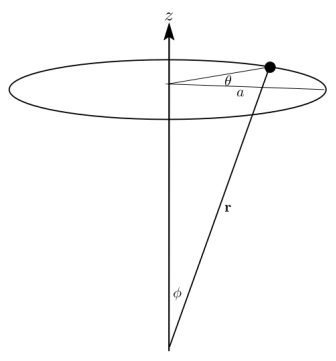
\includegraphics[trim=1.5 0 0 0, height=3.5cm,clip]{11_0.png}
	% 	% \caption{四个区域搜索空间}
  % \end{figure}
  
	\column{0.1\textwidth}

\end{columns}
\end{frame}

%%%%%%%%%%%%%%%%%%%%%%%%%%%%

\begin{frame}
  \frametitle{确定性误差分类 \hfill 
\includegraphics[height=0.5cm]{00_logo.png}}
  \begin{columns}
    \column{0.1\textwidth}
    
    \column{0.8\textwidth}
    \begin{enumerate}
      \item Bias \quad 理论上,当没有外界作用时,IMU的输出应该为0.但是,实际数据存在一个偏置b,加速度计bias对位姿估计的影响:
      \begin{equation}
        v_{err} = b^a t,\quad p_{err} = \frac{1}{2} b^a t^2        
      \end{equation}

      \item Scale \quad scale可以看成是理论数值和输出值之间的比值,如下图所示.
      \item Misalignment/Nonorthogonality Errors \quad 
      多轴IMU传感器制作的时候,由于制作工艺的问题,会使得xyz轴可能不垂直,如下图所示.

    \end{enumerate}

    \begin{figure}[h]
      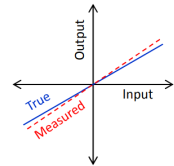
\includegraphics[trim=1.5 0 0 0, height=3.5cm,clip]{11_1.png}
      \qquad
      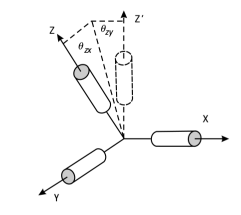
\includegraphics[trim=1.5 0 0 0, height=3.5cm,clip]{11_2.png}

      % \caption{四个区域搜索空间}
    \end{figure}
    % {\color{red}旋转矩阵是一个正交矩阵.它的行列式为1,且每个列向量都是单位向量且相互正交,它的逆等于它的转置.}
    
    \column{0.1\textwidth}
  
  \end{columns}
  \end{frame}   


% \section{IMU误差模型}

\begin{comment}
\end{comment}
\begin{frame}
\frametitle{确定性误差标定(六面法) \hfill 
\includegraphics[height=0.5cm]{00_logo.png}}
\begin{columns}
  \column{0.1\textwidth}
  
  \column{0.8\textwidth}
  % 六面法标定加速度计Bias/Scale和Nonorthogonality.

  六面法:将加速度计的3个轴分别朝上或朝下水平放置一段时间,采集6个面的数据完成标定.
	\begin{enumerate}
		\item 如果各个轴是正交的,那么很容易得到bias和scale:
		\begin{equation}
      \begin{split}
          &b = \frac{l^{up}_z + l^{down}_z}{2} \\
          & s = \frac{l^{up}_z - l^{down}_z}{2 \cdot ||g||}
      \end{split}
    \end{equation}

    其中,l为加速度计某个轴的测量值,g为当地的重力加速度.

  \end{enumerate}
  
  % \column{0.3\textwidth}
	% \begin{figure}[h]
	% 	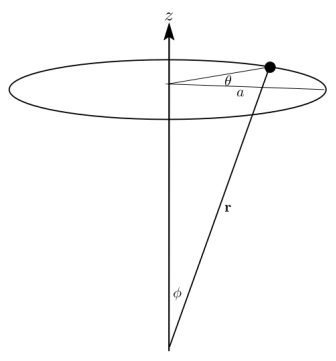
\includegraphics[trim=1.5 0 0 0, height=3.5cm,clip]{11_0.png}
	% 	% \caption{四个区域搜索空间}
  % \end{figure}
  
	\column{0.1\textwidth}

\end{columns}
\end{frame}

%%%%%%%%%%%%%%%%%%%%%%%%%%%%

\begin{comment}
\end{comment}
\begin{frame}
\frametitle{确定性误差标定(六面法) \hfill 
\includegraphics[height=0.5cm]{00_logo.png}}
\begin{columns}
  \column{0.1\textwidth}
  
  \column{0.8\textwidth}
  
  \begin{enumerate}
    \setcounter{enumi}{1}
		\item 考虑轴间误差的时候,实际加速度和测量值之间的关系为:
		\begin{equation}
      \begin{split}
        \begin{bmatrix}
          l_{ax} \\ l_{ay} \\ l_{az}
        \end{bmatrix} = 
        \begin{bmatrix}
          b_{ax} \\ b_{ay} \\ b_{az}
        \end{bmatrix} +
        \begin{bmatrix}
          s_{xx} & m_{xy} & m_{xz} \\
          m_{yx} & s_{yy} & m_{yz} \\
          m_{zx} & m_{zy} & s_{zz}
        \end{bmatrix} \cdot 
        \begin{bmatrix}
          a_x \\ a_y \\ a_z
        \end{bmatrix}
      \end{split}
    \end{equation}

    水平静止放置6面的时候,加速度的理论值为:

    \begin{equation}
      a1 = \begin{bmatrix}
        g \\ 0 \\ 0
      \end{bmatrix},
      a2 = \begin{bmatrix}
        -g \\ 0 \\ 0
      \end{bmatrix},
      a3 = \begin{bmatrix}
        0 \\ g \\ 0
      \end{bmatrix},
      a4 = \begin{bmatrix}
        0 \\ -g \\ 0
      \end{bmatrix},
      a5 = \begin{bmatrix}
        0 \\ 0 \\ g
      \end{bmatrix},
      a6 = \begin{bmatrix}
        0 \\ 0 \\ -g
      \end{bmatrix}
    \end{equation}

    其中,l为加速度计某个轴的测量值,g为当地的重力加速度.

    对应的测量值矩阵L:
    \begin{equation}
      L = [I_1, I_2,I_3,I_4,I_5, I_6]  
    \end{equation}

    利用最小二乘就能够把12个变量求出来.

  \end{enumerate}
  
  % \column{0.3\textwidth}
	% \begin{figure}[h]
	% 	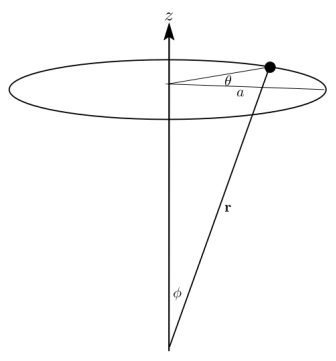
\includegraphics[trim=1.5 0 0 0, height=3.5cm,clip]{11_0.png}
	% 	% \caption{四个区域搜索空间}
  % \end{figure}
  
	\column{0.1\textwidth}

\end{columns}
\end{frame} 



%%%%%%%%%%%%%%%%%%%%%%%%%%%%

\begin{comment}
\end{comment}
\begin{frame}
\frametitle{确定性误差标定(六面法) \hfill 
\includegraphics[height=0.5cm]{00_logo.png}}
\begin{columns}
  \column{0.1\textwidth}
  
  \column{0.5\textwidth}
  六面法标定陀螺的bias,scale和misalignment.
  
  \begin{itemize}
    \item 和加速度计六面法不同的是,陀螺仪的真实值由高精度转台提供,这里的6面是指各个轴顺时针和逆时针旋转.
  \end{itemize}
  
  \column{0.3\textwidth}
	\begin{figure}[h]
		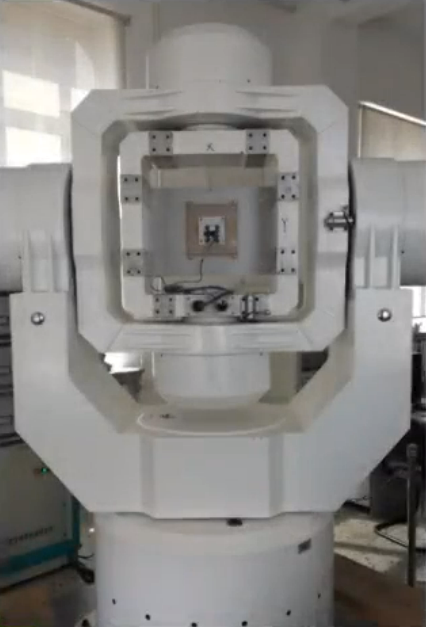
\includegraphics[trim=1.5 0 0 0, height=3.5cm,clip]{12_1.png}
		% \caption{四个区域搜索空间}
  \end{figure}
  
	\column{0.1\textwidth}

\end{columns}
\end{frame} 



% \section{IMU误差模型}

% \begin{comment}
% \end{comment}
% \begin{frame}
% \frametitle{确定性误差标定 \hfill 
\includegraphics[height=0.5cm]{00_logo.png}}
% \begin{columns}
%   \column{0.1\textwidth}
  
%   \column{0.8\textwidth}
%   IMU不依托额外设备实现标定

%   \begin{itemize}
%     \item aa
% %  \item 参考论文:[A Robust and Easy to Implement Method for IMU Calibration without External Equipments ](http://www.dis.uniroma1.it/~pretto/papers/tpm_icra2014.pdf)
  
%  \item DEMO链接:https://bitbucket.org/alberto_pretto/imu_tk
%   \end{itemize}


  
%   % \column{0.3\textwidth}
% 	% \begin{figure}[h]
% 	% 	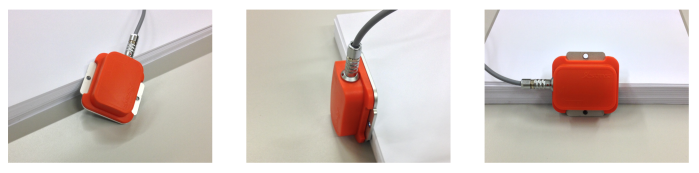
\includegraphics[trim=1.5 0 0 0, height=3.5cm,clip]{13_1.png}
% 	% 	% \caption{四个区域搜索空间}
%   % \end{figure}
  
% 	\column{0.1\textwidth}

% \end{columns}
% \end{frame}

%%%%%%%%%%%%%%%%%%%%%%%%%%%%

\begin{comment}
\end{comment}
\begin{frame}
\frametitle{IMU确定性误差标定(不依托额外设备法) \hfill 
\includegraphics[height=0.5cm]{00_logo.png}}
\begin{columns}
  \column{0.1\textwidth}
  
  \column{0.8\textwidth}
  
  \begin{itemize}
    % \item 参考论文:[A Robust and Easy to Implement Method for IMU Calibration without External Equipments ](http://www.dis.uniroma1.it/~pretto/papers/tpm_icra2014.pdf)
    \item 参考论文:\href{http://www.dis.uniroma1.it/~pretto/papers/tpm_icra2014.pdf}{A Robust and Easy to Implement Method for IMU Calibration without External Equipments} 
    \item DEMO链接:https://bitbucket.org/alberto\_pretto/imu\_tk
  \end{itemize}
  % \column{0.3\textwidth}
	\begin{figure}[h]
		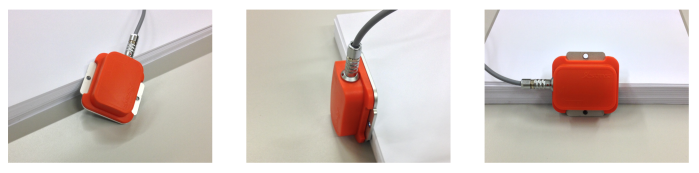
\includegraphics[trim=1.5 0 0 0, height=3.5cm,clip]{13_1.png}
		% \caption{四个区域搜索空间}
  \end{figure}
  
	\column{0.1\textwidth}

\end{columns}
\end{frame} 



%%%%%%%%%%%%%%%%%%%%%%%%%%%%

\begin{comment}
\end{comment}
\begin{frame}
\frametitle{IMU确定性误差标定(不依托额外设备法) \hfill 
\includegraphics[height=0.5cm]{00_logo.png}}
\begin{columns}
  \column{0.1\textwidth}
  
  \column{0.6\textwidth}
  
  IMU数据录制步骤:
  \begin{enumerate}
    \item Left the IMU static for 50 seconds.
    \item Rotate the IMU and then lay it in a different attitude.
    \item Wait for at least 1 seconds.
    \item Have you rotated the IMU 36 - 50 times? If not, go back to step 2.
    \item Done.
  \end{enumerate}
  
  \column{0.2\textwidth}
	\begin{figure}[h]
		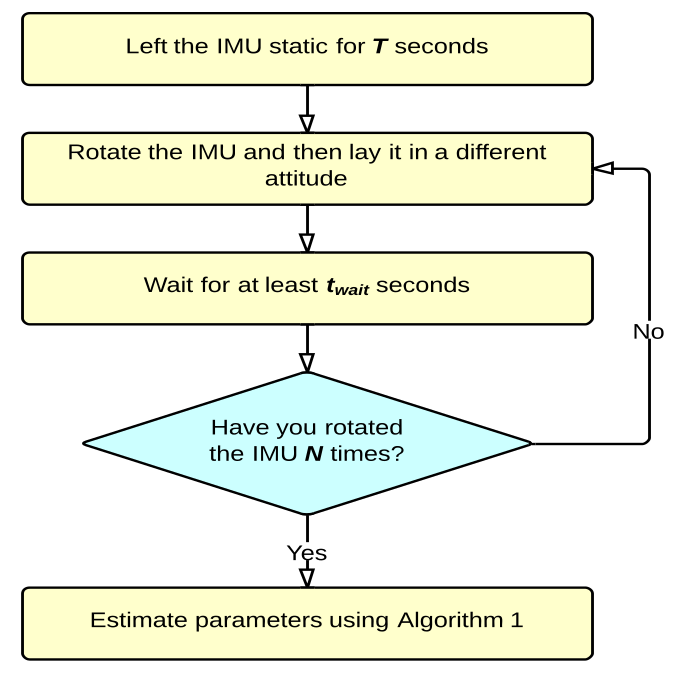
\includegraphics[trim=1.5 0 0 0, height=3.5cm,clip]{13_2.png}
		% \caption{四个区域搜索空间}
  \end{figure}
  
	\column{0.1\textwidth}

\end{columns}
\end{frame} 

%%%%%%%%%%%%%%%%%%%%%%%%%%%%

\begin{comment}
\end{comment}
\begin{frame}
\frametitle{IMU确定性误差标定(不依托额外设备法) \hfill 
\includegraphics[height=0.5cm]{00_logo.png}}
\begin{columns}
  \column{0.1\textwidth}
  
  \column{0.4\textwidth}
  % 确定性误差模型:
  % \begin{equation*}
  %   \begin{split}
  %     \begin{bmatrix}
  %       l_{ax} \\ l_{ay} \\ l_{az}
  %     \end{bmatrix} = 
  %     \begin{bmatrix}
  %       b_{ax} \\ b_{ay} \\ b_{az}
  %     \end{bmatrix} +
  %     \begin{bmatrix}
  %       s_{xx} & m_{xy} & m_{xz} \\
  %       m_{yx} & s_{yy} & m_{yz} \\
  %       m_{zx} & m_{zy} & s_{zz}
  %     \end{bmatrix} \cdot 
  %     \begin{bmatrix}
  %       a_x \\ a_y \\ a_z
  %     \end{bmatrix}
  %   \end{split}
  % \end{equation*}

  (IG1)加速度计确定性误差标定结果:
  \begin{figure}[h]
		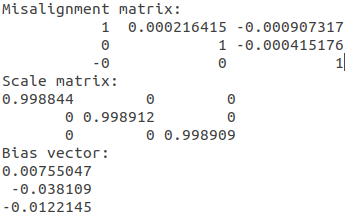
\includegraphics[trim=1.5 0 0 0, height=3.5cm,clip]{13_3.png}
		% \caption{四个区域搜索空间}
  \end{figure}
  
  % IMU确定性误差校正步骤:
  % \begin{enumerate}
  %   \item Left the IMU static for 50 seconds.
  %   \item Rotate the IMU and then lay it in a different attitude.
  %   \item Wait for at least 1 seconds.
  %   \item Have you rotated the IMU 36 ~ 50 times? If not, go back to step 2.
  %   \item Done.
  % \end{enumerate}
  
  \column{0.4\textwidth}
  (IG1)陀螺仪确定性误差标定结果:
	\begin{figure}[h]
		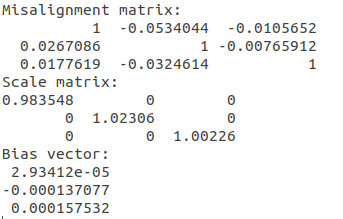
\includegraphics[trim=1.5 0 0 0, height=3.5cm,clip]{13_4.png}
		% \caption{四个区域搜索空间}
  \end{figure}
  
	\column{0.1\textwidth}

\end{columns}
\end{frame} 



\section{IMU随机误差模型及标定}

\begin{comment}
\end{comment}
\begin{frame}
\frametitle{IMU随机误差分类 \hfill 
\includegraphics[height=0.5cm]{00_logo.png}}
\begin{columns}
  \column{0.1\textwidth}
  
	\column{0.8\textwidth}
	\begin{enumerate}
		\item {\color{red}高斯白噪声} \quad		
		IMU数据连续时间上受到一个均值为0,方差为$\sigma$,各时刻之间相互独立的高斯过程$n(t)$:

\begin{equation}
  \begin{split}
    & E[n(t)] = 0 \\
    & E[n(t_1)n(t_2)] = \sigma^2 \delta(t1-t2)
  \end{split}
\end{equation}

其中,$\delta()$表示狄拉克函数.

	\item {\color{red}Bias随机游走}
	通常用维纳过程(wiener process)来建模bias随时间连续变化的过程,离散时间下称之为随机游走.

\begin{equation}
  \dot{b}(t) = n_b(t) = \sigma_b w(t)
\end{equation}

其中,$ w$是方差为1的白噪声.


\end{enumerate}
  
问题:实际上,IMU传感器产生的原始数据是连续的,而输出数据是离散的,离散和连续高斯白噪声存在何种关系?

  % \column{0.3\textwidth}
	% \begin{figure}[h]
	% 	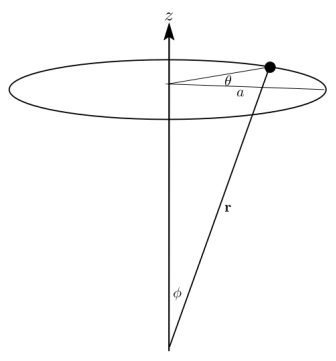
\includegraphics[trim=1.5 0 0 0, height=3.5cm,clip]{11_0.png}
	% 	% \caption{四个区域搜索空间}
  % \end{figure}
  
	\column{0.1\textwidth}

\end{columns}
\end{frame}

%%%%%%%%%%%%%%%%%%%%%%%%%%%%

\begin{frame}
  \frametitle{高斯白噪声的离散化 \hfill 
\includegraphics[height=0.5cm]{00_logo.png}}
  \begin{columns}
    \column{0.1\textwidth}
    
    \column{0.8\textwidth}

    只考虑高斯白噪声的积分
    \begin{equation}
      n_d[k] \triangleq n(t_0 + \Delta t) \simeq \frac{1}{\Delta t} \int ^{t_0+\Delta t}_{t_0} n(t) dt
    \end{equation}

    协方差为:
    \begin{equation}
      \begin{split}
        E(n^2_d[k]) &= E(\frac{1}{\Delta t^2} \int ^{t_0+\Delta t}_{t_0} \int ^{t_0+\Delta t}_{t_0} n(\tau) n(t))d\tau dt \\
        &= \frac{1}{\Delta t^2} \int ^{t_0+\Delta t}_{t_0} \int ^{t_0+\Delta t}_{t_0} E(n(\tau) n(t))d\tau dt \\
        &= \frac{\sigma^2}{\Delta t^2} \int ^{t_0+\Delta t}_{t_0} \int ^{t_0+\Delta t}_{t_0} \delta(t-\tau)d\tau dt \\
        &= \frac{\sigma^2}{\Delta t}        
      \end{split}
    \end{equation}
    
    \column{0.1\textwidth}
  
  \end{columns}
  \end{frame}   

%%%%%%%%%%%%%%%%%%%%%%%%%%%%

\begin{frame}
  \frametitle{高斯白噪声的离散化 \hfill 
\includegraphics[height=0.5cm]{00_logo.png}}
  \begin{columns}
    \column{0.1\textwidth}
    
    \column{0.8\textwidth}

    即:
    \begin{equation}
      n_d[k] = \sigma w[k]
    \end{equation}

    其中,
    \begin{equation}
      \begin{split}
        &w[k] \sim N(0, 1) \\
        &\sigma_d = \sigma \frac{1}{\Delta t}
      \end{split}
    \end{equation}
    
    也就是说高斯白噪声的连续时间表示到离散时间表示相差一个$\frac{1}{\Delta t}$,$\sqrt{\Delta t}$是传感器的采样时间.

    \column{0.1\textwidth}
  
  \end{columns}
  \end{frame}   

%%%%%%%%%%%%%%%%%%%%%%%%%%%%

\begin{frame}
  \frametitle{bias随机游走的离散化 \hfill 
\includegraphics[height=0.5cm]{00_logo.png}}
  \begin{columns}
    \column{0.1\textwidth}
    
    \column{0.8\textwidth}

    

      提取bias积分部分

      \begin{equation}
        b(t_0+\Delta t) = b(t_0) + \int ^{t_0+\Delta t}_{t_0} n_b(t) dt  
      \end{equation}

      由此可得离散化下的bias协方差:
      \begin{equation}
        E\{b^2(t_0+\Delta t)\} = E\{[b(t_0)+\int ^{t_0+\Delta t}_{t_0}n_b(t)dt][b(t_0)+\int ^{t_0+\Delta t}_{t_0}n_b(\tau)d\tau]\}  
      \end{equation}

      由于$E\{n_b(t)n_b(\tau)\} = \sigma^2_b \delta(t-\tau)$有:
      \begin{equation}
        E\{b^2(t_0+\Delta t)\} = E\{b^2(t_0)\} + \sigma^2_b \Delta t
      \end{equation}
    
    \column{0.1\textwidth}
  
  \end{columns}
  \end{frame}     


  %%%%%%%%%%%%%%%%%%%%%%%%%%%%

\begin{frame}
  \frametitle{bias随机游走的离散化 \hfill 
\includegraphics[height=0.5cm]{00_logo.png}}
  \begin{columns}
    \column{0.1\textwidth}
    
    \column{0.8\textwidth}

    即:
\begin{equation}
  b_d[k] = b_d[k-1] + \sigma_{bd}w[k]
\end{equation}

其中,
\begin{equation}
  \begin{split}
    & w[k] \sim N(0, 1)\\
    & \sigma_{bd} = \sigma_b \sqrt{\Delta t}
  \end{split}
\end{equation}

  bias随机游走的噪声方差从连续时间到离散之间需要乘以$\sqrt{\Delta t}$
    
    \column{0.1\textwidth}
  
  \end{columns}
  \end{frame}    

%   %%%%%%%%%%%%%%%%%%%%%%%%%%%%

% \begin{frame}
%   \frametitle{高斯白噪声的离散化 \hfill 
\includegraphics[height=0.5cm]{00_logo.png}}
%   \begin{columns}
%     \column{0.1\textwidth}
    
%     \column{0.8\textwidth}

%     只考虑高斯白噪声的积分
%     \begin{equation}
%       n_d[k] \triangleq n(t_0 + \Delta t) \simeq \frac{1}{\Delta t} \int ^{t_0+\Delta t}_{t_0} n(t) dt
%     \end{equation}

%     协方差为:
%     \begin{equation}
%       \begin{split}
%         E(n^2_d[k]) &= E(\frac{1}{\Delta t^2} \int ^{t_0+\Delta t}_{t_0} \int ^{t_0+\Delta t}_{t_0} n(\tau) n(t))d\tau dt \\
%         &= \frac{1}{\Delta t^2} \int ^{t_0+\Delta t}_{t_0} \int ^{t_0+\Delta t}_{t_0} E(n(\tau) n(t))d\tau dt \\
%         &= \frac{\sigma^2}{\Delta t^2} \int ^{t_0+\Delta t}_{t_0} \int ^{t_0+\Delta t}_{t_0} \delta(t-\tau)d\tau dt \\
%         &= \frac{\sigma^2}{\Delta t}        
%       \end{split}
%     \end{equation}
    
%     \column{0.1\textwidth}
  
%   \end{columns}
%   \end{frame}    


 

%%%%%%%%%%%%%%%%%%%%%%%%%%%%

\begin{comment}
\end{comment}
\begin{frame}
\frametitle{IMU随机误差标定 \hfill 
\includegraphics[height=0.5cm]{00_logo.png}}
\begin{columns}
  \column{0.1\textwidth}
  
  \column{0.8\textwidth}
  

  \begin{itemize}
    % \item 参考论文:[A Robust and Easy to Implement Method for IMU Calibration without External Equipments ](http://www.dis.uniroma1.it/~pretto/papers/tpm_icra2014.pdf)
    \item 参考
    \begin{enumerate}
      \item An introduction to inertial navigation
      \item Allan Variance: Noise Analysis for Gyroscopes
      \item DEMO:https://github.com/gaowenliang/imu\_utils
    \end{enumerate}

    \item IMU数据录制步骤:
    \begin{enumerate}
      \item 保持imu静止不动至少2个小时.
    \end{enumerate}
    
  \end{itemize}
  % % \column{0.3\textwidth}
	% \begin{figure}[h]
	% 	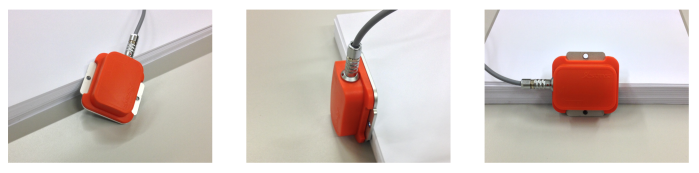
\includegraphics[trim=1.5 0 0 0, height=3.5cm,clip]{13_1.png}
	% 	% \caption{四个区域搜索空间}
  % \end{figure}
  
	\column{0.1\textwidth}

\end{columns}
\end{frame} 



% %%%%%%%%%%%%%%%%%%%%%%%%%%%%

% \begin{comment}
% \end{comment}
% \begin{frame}
% \frametitle{IMU确定性误差标定(不依托额外设备法) \hfill 
\includegraphics[height=0.5cm]{00_logo.png}}
% \begin{columns}
%   \column{0.1\textwidth}
  
%   \column{0.6\textwidth}
  
% 	\begin{figure}[h]
% 		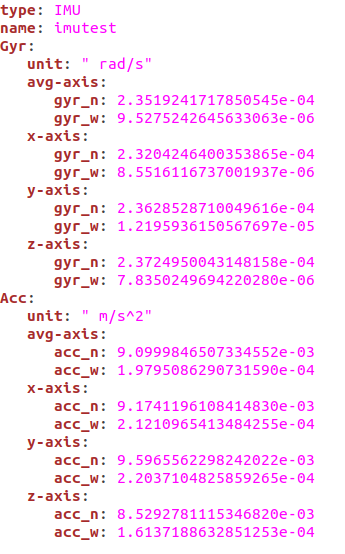
\includegraphics[trim=1.5 0 0 0, height=3.5cm,clip]{22_1.png}
% 		% \caption{四个区域搜索空间}
%   \end{figure}
  
% 	\column{0.1\textwidth}

% \end{columns}
% \end{frame} 

%%%%%%%%%%%%%%%%%%%%%%%%%%%%

\begin{comment}
\end{comment}
\begin{frame}
\frametitle{IMU随机误差标定 \hfill 
\includegraphics[height=0.5cm]{00_logo.png}}
\begin{columns}
  \column{0.1\textwidth}
  
  \column{0.4\textwidth}
  % 确定性误差模型:
  % \begin{equation*}
  %   \begin{split}
  %     \begin{bmatrix}
  %       l_{ax} \\ l_{ay} \\ l_{az}
  %     \end{bmatrix} = 
  %     \begin{bmatrix}
  %       b_{ax} \\ b_{ay} \\ b_{az}
  %     \end{bmatrix} +
  %     \begin{bmatrix}
  %       s_{xx} & m_{xy} & m_{xz} \\
  %       m_{yx} & s_{yy} & m_{yz} \\
  %       m_{zx} & m_{zy} & s_{zz}
  %     \end{bmatrix} \cdot 
  %     \begin{bmatrix}
  %       a_x \\ a_y \\ a_z
  %     \end{bmatrix}
  %   \end{split}
  % \end{equation*}

  (IG1)加速度计随机性误差标定结果:
  \begin{figure}[h]
		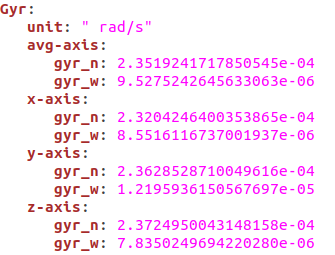
\includegraphics[trim=1.5 0 0 0, height=3.5cm,clip]{22_2.png}
		% \caption{四个区域搜索空间}
  \end{figure}
  
  % IMU确定性误差校正步骤:
  % \begin{enumerate}
  %   \item Left the IMU static for 50 seconds.
  %   \item Rotate the IMU and then lay it in a different attitude.
  %   \item Wait for at least 1 seconds.
  %   \item Have you rotated the IMU 36 ~ 50 times? If not, go back to step 2.
  %   \item Done.
  % \end{enumerate}
  
  \column{0.4\textwidth}
  (IG1)陀螺仪随机性误差标定结果:
	\begin{figure}[h]
		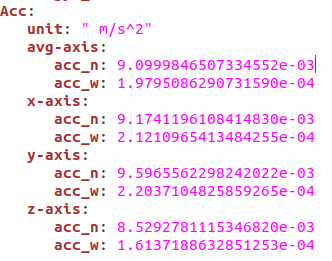
\includegraphics[trim=1.5 0 0 0, height=3.5cm,clip]{22_3.png}
		% \caption{四个区域搜索空间}
  \end{figure}
  
	\column{0.1\textwidth}

\end{columns}
\end{frame} 





\begin{comment}
\end{comment}
\begin{frame}
\frametitle{Reference \hfill 
\includegraphics[height=0.5cm]{00_logo.png}}
\begin{columns}
  \column{0.1\textwidth}
  
  \column{0.8\textwidth}
	% \begin{enumerate}
	% 	\item 如果各个轴是正交的,那么很容易得到bias和scale:
	% \end{enumerate}
	[1] 如果各个轴是正交的
  
  % \column{0.3\textwidth}
	% \begin{figure}[h]
	% 	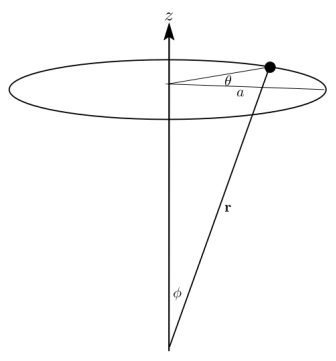
\includegraphics[trim=1.5 0 0 0, height=3.5cm,clip]{11_0.png}
	% 	% \caption{四个区域搜索空间}
  % \end{figure}
  
	\column{0.1\textwidth}

\end{columns}
\end{frame}

%%%%%%%%%%%%%%%%%%%%%%%%%%%%

% \section{IMU测量模型}
\subsection{加速度计测量原理}
\subsection{陀螺仪的测量原理}

%%%%%%%%%%%%%%%%%%%%%%%%%%%%

\begin{frame}
  \frametitle{加速度计测量原理 \hfill 
\includegraphics[height=0.5cm]{00_logo.png}}
  \begin{columns}
    \column{0.1\textwidth}
    
    \column{0.5\textwidth}
    \begin{itemize}
      \item 其测量原理可以用一个质量块+弹簧+指示计来表示.
      \item 加速度计测量值$a_m$为弹簧拉力对应的加速度,
        \begin{equation}
          a_m = \frac{f}{m} = a - g
        \end{equation}
      
      其中,f为弹簧拉力, a为物体在惯性系下的加速度,g为重力加速度.
      
      \item 通过受力影响位移,位移影响电容大小,通过测量电流的方式获得$a_m$

    \end{itemize}

    \column{0.3\textwidth}
    \begin{figure}[h]
      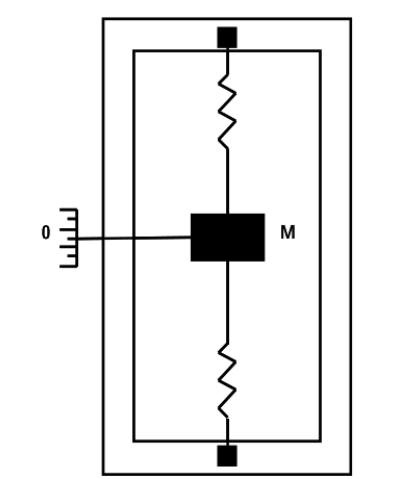
\includegraphics[trim=1.5 0 0 0, height=3.5cm,clip]{12_0.png}
      % \caption{四个区域搜索空间}
    \end{figure}

    \column{0.1\textwidth}
  
  \end{columns}
  \end{frame}    


%%%%%%%%%%%%%%%%%%%%%%%%%%%%

\begin{frame}
  \frametitle{陀螺仪测量原理 \hfill 
\includegraphics[height=0.5cm]{00_logo.png}}
  \begin{columns}
    \column{0.1\textwidth}
    
    \column{0.5\textwidth}
    \begin{itemize}
      \item 陀螺仪主要用来测量物体的旋转角速度,按测量原理分有震动陀螺/光纤陀螺等.

      \item 一般采用震动陀螺原理,通过测量Coriolis force 来间接得到角速度.
      
      \item 一个主动运动轴 + 一个敏感轴

    \end{itemize}
    
    \column{0.3\textwidth}
    \begin{figure}[h]
      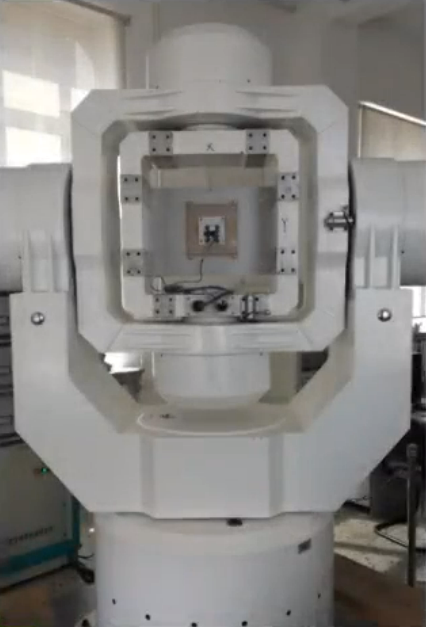
\includegraphics[trim=1.5 0 0 0, height=3.5cm,clip]{12_1.png}
      % \caption{四个区域搜索空间}
    \end{figure}

    \column{0.1\textwidth}
  
  \end{columns}
  \end{frame}    

%%%%%%%%%%%%%%%%%%%%%%%%%%%%

\begin{frame}
  \frametitle{音叉振动陀螺原理 \hfill 
\includegraphics[height=0.5cm]{00_logo.png}}
  \begin{columns}
    \column{0.1\textwidth}
    
    \column{0.8\textwidth}
    \begin{itemize}
      \item 音叉中间为旋转轴,音叉左右两个质量块,做方向相反的正弦运动,质量块受到的科氏力方向相反.
      \item 为什么要这么做?一个质量块行不行?

    \end{itemize}
    
    % \column{0.4\textwidth}
    \begin{figure}[h]
      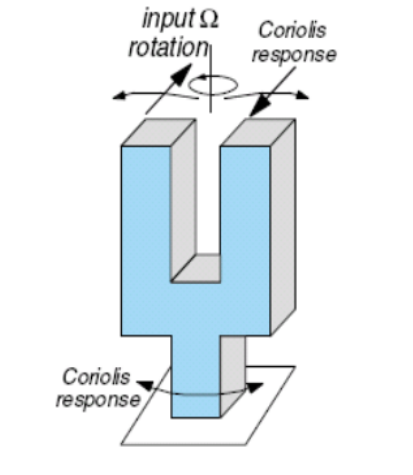
\includegraphics[trim=1.5 0 0 0, height=3.5cm,clip]{12_2.png}
      \qquad
      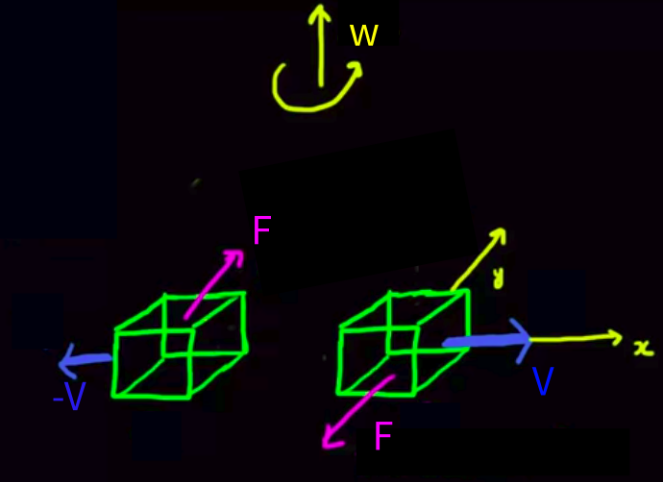
\includegraphics[trim=1.5 0 0 0, height=3.5cm,clip]{12_3.png}
      % \caption{四个区域搜索空间}
    \end{figure}

    \column{0.1\textwidth}
  
  \end{columns}
  \end{frame}    

%%%%%%%%%%%%%%%%%%%%%%%%%%%%

\begin{frame}
  \frametitle{思考 \hfill 
\includegraphics[height=0.5cm]{00_logo.png}}
  \begin{columns}
    \column{0.1\textwidth}
    
    \column{0.8\textwidth}
    \begin{itemize}
      \item 实际上,两个质量块不可能完全一致,也就是说陀螺仪的测量会受到外部加速度的影响,即常称的G-sensitivity.
      
      \item 加速度计不需要考虑科氏力的影响吗?

    \end{itemize}
    

    \column{0.1\textwidth}
  
  \end{columns}
  \end{frame}    
% \input{contents/22_IMU测量模型.tex}
% % \section{IMU误差模型}
\section{近期IMU应用中的问题及解决}

%%%%%%%%%%%%%%%%%%%%%%%%%%%%

\begin{frame}[fragile]
  \frametitle{近期IMU应用中的问题及解决(一) \hfill 
\includegraphics[height=0.5cm]{00_logo.png}}
  \begin{columns}
    \column{0.1\textwidth}
    
    \column{0.8\textwidth}
    \begin{itemize}
      \item 问题一:同样是右手坐标系,不同的是$z$轴上的数值取反(原来重力大小为-9.8,需要改成9.8),有两种方式.

      \item 方式一:
      
      \begin{lstlisting}[frame=shadowbox]  
        // pentu_ig1.urdf
        <joint name="imu_link_joint" type="fixed">
          <parent link="base_footprint" />
          <child link="imu" />
          <origin xyz="0 0 0" rpy="3.14 0 0"/>
        </joint>
      \end{lstlisting}

      \begin{lstlisting}[frame=shadowbox]  
        // SensorBridge::HandleImuMessage()
        imu_data->angular_velocity = Eigen::Vector3d{imu_data->angular_velocity[0], 
            -imu_data->angular_velocity[1], -imu_data->angular_velocity[2]};
        imu_data->linear_acceleration = Eigen::Vector3d{imu_data->linear_acceleration[0],
            -imu_data->linear_acceleration[1], imu_data->linear_acceleration[2]};    
        ......    
        trajectory_builder_->AddSensorData( sensor_id,
            carto::sensor::ImuData{imu_data->time, imu_data->linear_acceleration,
                               imu_data->angular_velocity});
      \end{lstlisting}

    \end{itemize}
    
    % \column{0.3\textwidth}
    % \begin{figure}[h]
    %   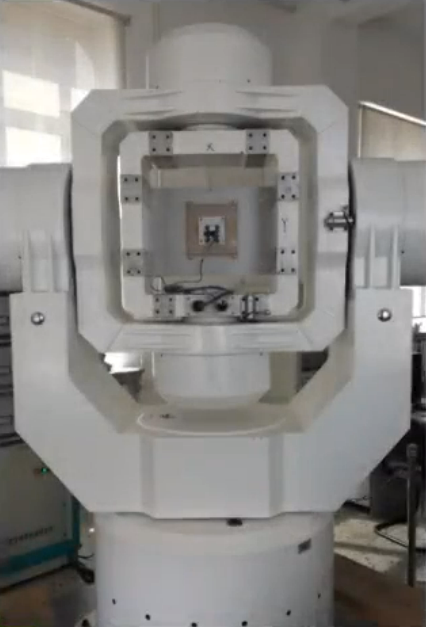
\includegraphics[trim=1.5 0 0 0, height=3.5cm,clip]{12_1.png}
    %   % \caption{四个区域搜索空间}
    % \end{figure}

    \column{0.1\textwidth}
  
  \end{columns}
  \end{frame}   

  %%%%%%%%%%%%%%%%%%%%%%%%%%%%

\begin{frame}[fragile]
  \frametitle{近期IMU应用中的问题及解决(一) \hfill \includegraphics[height=0.5cm]{00_logo.png}}
  \begin{columns}
    \column{0.1\textwidth}
    
    \column{0.8\textwidth}
    \begin{itemize}
      \item 方式二:
      
      \begin{lstlisting}[frame=shadowbox]  
        // pentu_ig1.urdf
        <joint name="imu_link_joint" type="fixed">
          <parent link="base_footprint" />
          <child link="imu" />
          <origin xyz="0 0 0" rpy="0 0 0"/>
        </joint>
      \end{lstlisting}

      \begin{lstlisting}[frame=shadowbox]  
        // SensorBridge::HandleImuMessage()
        imu_data->linear_acceleration[2] = -imu_data->linear_acceleration[2];    
        ......    
        trajectory_builder_->AddSensorData( sensor_id,
            carto::sensor::ImuData{imu_data->time, imu_data->linear_acceleration,
                               imu_data->angular_velocity});
      \end{lstlisting}

    \end{itemize}
    
    % \column{0.3\textwidth}
    % \begin{figure}[h]
    %   \includegraphics[trim=1.5 0 0 0, height=3.5cm,clip]{12_1.png}
    %   % \caption{四个区域搜索空间}
    % \end{figure}

    \column{0.1\textwidth}
  
  \end{columns}
  \end{frame}   


  %%%%%%%%%%%%%%%%%%%%%%%%%%%%

\begin{frame}[fragile]
  \frametitle{近期IMU应用中的问题及解决(二) \hfill \includegraphics[height=0.5cm]{00_logo.png}}
  \begin{columns}
    \column{0.1\textwidth}
    
    \column{0.8\textwidth}
    \begin{itemize}
      \item 问题二:IMU安装不是不水平的,base\_footprint到imu的静态TF的标定困难.解决方法是开发一个自动标定IMU的代码.

      
      \begin{lstlisting}[frame=shadowbox]  
        // pentu_ig1.urdf
        <joint name="imu_link_joint" type="fixed">
          <parent link="base_footprint" />
          <child link="imu" />
          <origin xyz="0 0 0" rpy="-0.00478014 -0.000399168 0"/>
        </joint>

      \end{lstlisting}

    \end{itemize}
    
    % \column{0.3\textwidth}
    % \begin{figure}[h]
    %   \includegraphics[trim=1.5 0 0 0, height=3.5cm,clip]{12_1.png}
    %   % \caption{四个区域搜索空间}
    % \end{figure}

    \column{0.1\textwidth}
  
  \end{columns}
  \end{frame}   

%%%%%%%%%%%%%%%%%%%%%%%%%%%%

\begin{frame}[fragile]
  \frametitle{近期IMU应用中的问题及解决(二) \hfill \includegraphics[height=0.5cm]{00_logo.png}}
  \begin{columns}
    \column{0.1\textwidth}
    
    \column{0.8\textwidth}
      \begin{lstlisting}[frame=shadowbox]  
        void ImuCallback(const sensor_msgs::ImuConstPtr& msg)
        {
          static int nums = 0;
          static Eigen::Vector3d calibr_sum;
          if(++nums > 500)
            return;
          if(nums <= 500)
          {
            std::unique_ptr<cartographer::sensor::ImuData> imu_data = ToImuData(msg);
            const Eigen::Quaterniond rotation = Eigen::Quaterniond::FromTwoVectors(
              imu_data->linear_acceleration, Eigen::Vector3d{0, 0, -9.8});  
            Eigen::Vector3d calibr = cartographer::transform::RotationQuaternionToAngleAxisVector(rotation);
            calibr_sum += calibr;
          }
          if(nums == 500)
              std::cout << "[rpy:]" << calibr_sum / 500 << std::endl;
        }
      \end{lstlisting}

    
    % \column{0.3\textwidth}
    % \begin{figure}[h]
    %   \includegraphics[trim=1.5 0 0 0, height=3.5cm,clip]{12_1.png}
    %   % \caption{四个区域搜索空间}
    % \end{figure}

    \column{0.1\textwidth}
  
  \end{columns}
  \end{frame}   





% \begin{frame}[plain]{}
%   \begin{center}
%     \begin{tikzpicture}
%       \node[above,xscale=1.2,yscale=1.2]{\Huge 欢迎批评指正!};
%     \end{tikzpicture}
%   \end{center}
% \end{frame}
% -----------------------------------------------------------
\begin{frame}[plain]{}
  \begin{center}
    \begin{tikzpicture}
      \node[above,xscale=1.2,yscale=1.2]{\Huge {\color{red}{感谢聆听!!!}}};
    \end{tikzpicture}
  \end{center}
\end{frame}

% {\color{red}第一期:旋转运动学 ;\quad IMU测量模型}

\end{document}
